\clearpage
\section{Arithmetic Encoding \& Decoding}

\begin{refsection}

\begin{tcolorbox}	
\begin{tabular}{p{2.75cm} p{0.2cm} p{10.5cm}} 	
\textbf{Students Name}  &:& Diogo Barros (46084) \\
\textbf{Starting Date} &:& July 17, 2018\\
\textbf{Goal}          &:& Integer implementation of Arithmetic encoding and decoding.
\end{tabular}
\end{tcolorbox}

Arithmetic encoding is a source coding technique that represents a complete string as a real number in a sub-interval of the unit interval [0,1). Since this interval has unlimited real numbers, it is possible to assign an unique real number to any string of a given length. The coded string is the binary representation of the assigned real value.

Unlike Huffman encoding, a unique code is obtained without the need to generate all codes of all possible strings of the same length, though the implementation of arithmetic coding is significantly more complex to circumvent numeric precision problems.

\subsection{Encoding Algorithm}

\begin{tcolorbox}	
	\begin{tabular}{p{2.75cm} p{0.2cm} p{10.5cm}} 	
		\textbf{Students Name}  &:& Diogo Barros (17/07/2018 - 20/07/2018)\\
		\textbf{Goal}          &:& Arithmetic Encoding Algorithm Description
	\end{tabular}
\end{tcolorbox}

The first reference to arithmetic encoding was made in~\cite{Abramson63}. However, the first practical implementations were only proposed in 1976 by Pasco~\cite{Pasco76} and Rissanen~\cite{Rissanen76}. The block diagram of the algorithm in it's most simple floating point formulation is presented in Fig. \ref{fig:arithEncBlockDiagr}.

\begin{figure}[t]
	\centering
	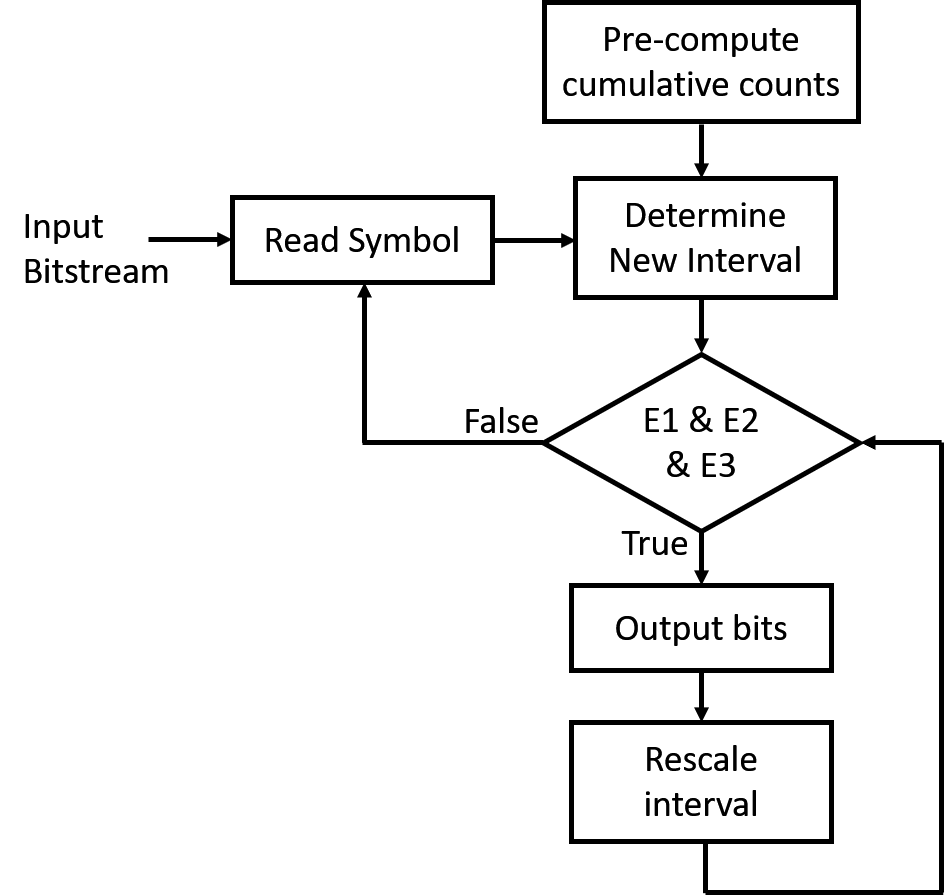
\includegraphics[width=0.6\textwidth]{./sdf/eit_46084_arithmetic_encoder_decoder/figures/ArithEncoderBlockDiagram.png}
	\caption{Block diagram of the algorithm for arithmetic encoding.} \label{fig:arithEncBlockDiagr}
\end{figure}

The first step before the encoding starts is to compute the cumulative symbol probabilities of the source, given the probabilities of each individual symbol. The initial interval is set to [0,1) and is subdivided into sub intervals based on the symbol probabilities. The required resolution (number of bits) of the registers that represent the limits of the current interval is given by the lowest symbol probability as expressed in (\ref{eq:resolEq})
\begin{equation} \label{eq:resolEq}
	Resolution = \lceil(-\log_2(\min(P(x_n))))\rceil + 1
\end{equation}

The encoding process starts by reading a symbol, identifying the corresponding sub interval in the current interval and updating the variables that save the current interval limits by using (\ref{eq:updateInterval1})-(\ref{eq:updateInterval3}).
\begin{eqnarray}
\label{eq:updateInterval1} &delta = lim\_high - lim\_low + 1 \\
&lim\_high = lim\_low + \lfloor delta \cdot count(symb + 1) / total\_count \rfloor - 1 \\
\label{eq:updateInterval3} &lim\_low = lim\_low + \lfloor delta \cdot count(symb) / total\_count \rfloor
\end{eqnarray}

At this point we need to perform two operations. The first is to check if we are able to output any code bit. The second is to rescale the interval if its amplitude is small enough. These operations are done based on the three conditions (\ref{eq:E1}), (\ref{eq:E2}) and (\ref{eq:E3}). The algorithm keeps track of how many times condition (\ref{eq:E3}) is met in succession and increments an internal extra bit counter.
\begin{eqnarray}
\label{eq:E1} &E1 = (lim\_low < 0.5) \  \&\& \ (lim\_high < 0.5) \\
\label{eq:E2} &E2 = (lim\_low > 0.5) \ \&\& \ (lim\_high > 0.5) \\
\label{eq:E3} &E3 = (lim\_low > 0.25) \ \&\& \ (lim\_high < 0.75)
\end{eqnarray}

When (\ref{eq:E1}) is met, the algorithm outputs a '0' and a number of extra '1' bits equal to the number of times (\ref{eq:E3}) was met previously and the extra bit counter is reset. When (\ref{eq:E1}) is met, the algorithm outputs a '1' and a number of '0' bits equal to the number of times (\ref{eq:E3}) was met previously and the extra bit counter is reset. In the practical implementation, these conditions are tested by comparing the most significant bits of each register.

If any of these conditions is met, the amplitude of the interval is lower than $0.25$ and needs to be rescaled by a factor of two, depending on which condition is met, as described in (\ref{eq:E1scale}), (\ref{eq:E2scale}) and (\ref{eq:E3scale}).
\begin{eqnarray}
\label{eq:E1scale} &E1:\ lim\_low = 2 \cdot lim\_low;\ lim\_high = 2 \cdot lim\_high;\\
\label{eq:E2scale} &E2:\ lim\_low = 2 \cdot (lim\_low-0.5);\ lim\_high = 2 \cdot (lim\_high-0.5); \\
\label{eq:E3scale} &E3:\ lim\_low = 2 \cdot (lim\_low-0.25);\ lim\_high = 2 \cdot (lim\_high-0.25);
\end{eqnarray}

The interval keeps on rescaling until none of the conditions is met, after which a new symbol is read and the process repeats until all symbols are coded.

% \cite{Abramson63} \cite{Pasco76} \cite{Rissanen76}

%%%%%%%%%%%%%%%%%%%%%%%%%%%%%%%%%%%%%%%%%%%%%%%%%%%%%%%%%%%%%%%%%%%%%%%%%%%%%%%%%%%%%%

\subsection{Decoding Algorithm}

\begin{tcolorbox}	
\begin{tabular}{p{2.75cm} p{0.2cm} p{10.5cm}} 	
\textbf{Students Name}  &:& Diogo Barros (18/07/2018 - 20/07/2018) \\
\textbf{Goal}          &:& Arithmetic Decoding Algorithm Description.
\end{tabular}
\end{tcolorbox}

The decoding operations are the same as the ones performed by the coding algorithm with the exception of symbol identification and how the output bits are determined. The simplified block diagram of the encoder algorithm is presented in Fig. \ref{fig:arithDecBlockDiagr}.

The decoder uses the same bit resolution as that of the encoder and starts by reading that number of bits from the coded bit stream, that becomes the "tag" value. The tag is then normalized as expressed in (\ref{eq:tagnorm}) and used to find the next symbol that was coded. This is done by finding the interval in the cumulative probability vector that contains it. Once the symbol is identified the code that corresponds to it can be sent to the output.
\begin{equation} \label{eq:tagnorm}
tag\_norm = \lfloor((tag - lim\_low + 1) \cdot total\_count - 1) / (lim\_high - lim\_low + 1)\rfloor
\end{equation}

The interval is updated in the same way as in the encoder and the conditions (\ref{eq:E1}), (\ref{eq:E2}) and (\ref{eq:E3}) are computed to rescale the interval. Additionally the tag value is updated based on which of these conditions is met.

\begin{figure}[H]
	\centering
	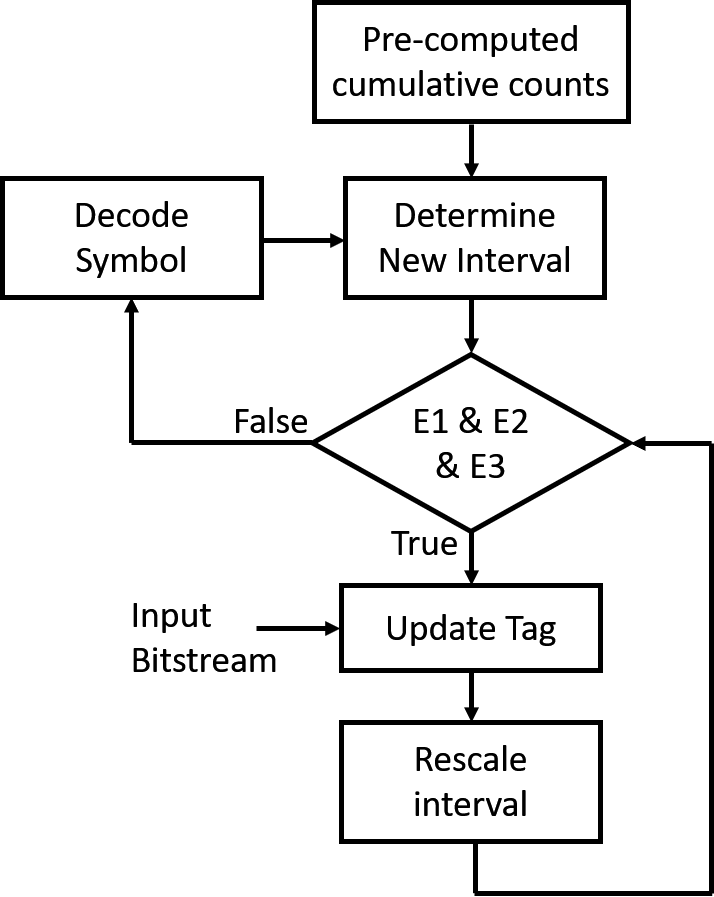
\includegraphics[width=0.5\textwidth]{./sdf/eit_46084_arithmetic_encoder_decoder/figures/ArithDecoderBlockDiagram.png}
	\caption{Block diagram of the algorithm for arithmetic decoding.} \label{fig:arithDecBlockDiagr}
\end{figure}

If either (\ref{eq:E1}) or (\ref{eq:E2}) is met, a new bit is read from the coded bit stream and added to the tag value multiplied by two. In the implemented code this is done right shifting the tag bits by one (discarding the most significant bit) and adding the new bit to it. If (\ref{eq:E3}) is met, the tag is updated in the same way but the new most significant bit is negated. When none of the conditions is met, a new symbol is decoded using the tag value normalized and the process continues until all symbols are decoded.


\subsection{Encoding and Decoding Simulation Results}

To test the implemented encoding and decoding algorithms, the system presented in Fig.\ref{fig:SystemBlockDiagr} was created in simulation. The system contains a binary source, the arithmetic encoding and decoding blocks and a bit-error-ratio computation block to ensure that the information is not degraded.

\begin{figure}[h]
	\centering
	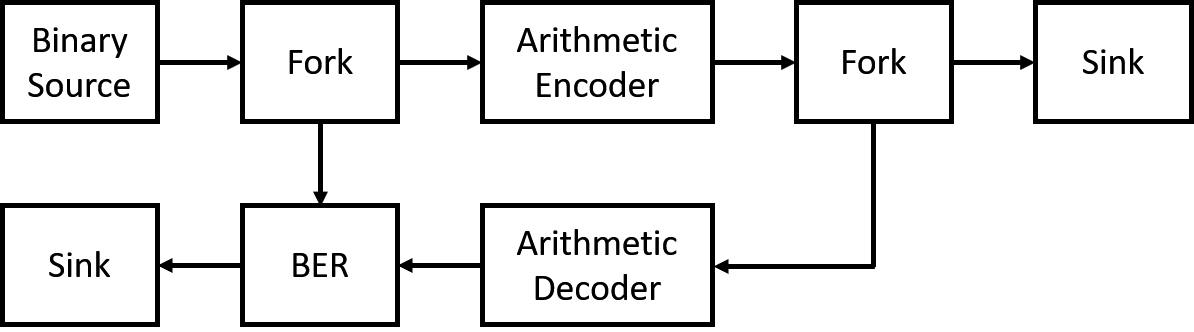
\includegraphics[width=0.85\textwidth]{./sdf/eit_46084_arithmetic_encoder_decoder/figures/TestSystemBlockDiagram.png}
	\caption{Block diagram of the floating point algorithm for arithmetic decoding.}\label{fig:SystemBlockDiagr}
\end{figure}

A test simulation with a total of 45360 bits and a probability of zero of 0.1 was performed. the number of bits of the encoder was changed from 2 to 5 and the code efficiency, given by (\ref{eq:codeEff}), was computed for each value. The results are presented in Fig.\ref{fig:CodeEff}. As expected, the code efficiency of the arithmetic algorithm is very close to optimum and increases as the number of coding bits increases.
\begin{equation} \label{eq:codeEff}
\eta = \frac{H(n)}{L}
\end{equation}

\begin{figure}[h]
	\centering
	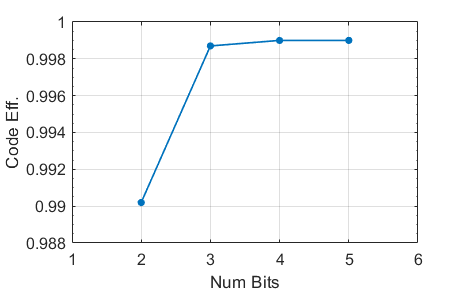
\includegraphics[width=0.65\textwidth]{./sdf/eit_46084_arithmetic_encoder_decoder/figures/CodeEff.png}
	\caption{Code efficiency variation with the number of coding bits.} \label{fig:CodeEff}
\end{figure}


\newpage

% bibliographic references for the section ----------------------------
\clearpage
%\printbibliography[heading=subbibliography]
\end{refsection}
\addcontentsline{toc}{subsection}{Bibliography}
\cleardoublepage
% --------------------------------------------------------------------- 